\documentclass[preview]{standalone}
\usepackage{tikz}

\begin{document}

\begin{figure}[ht]
\center
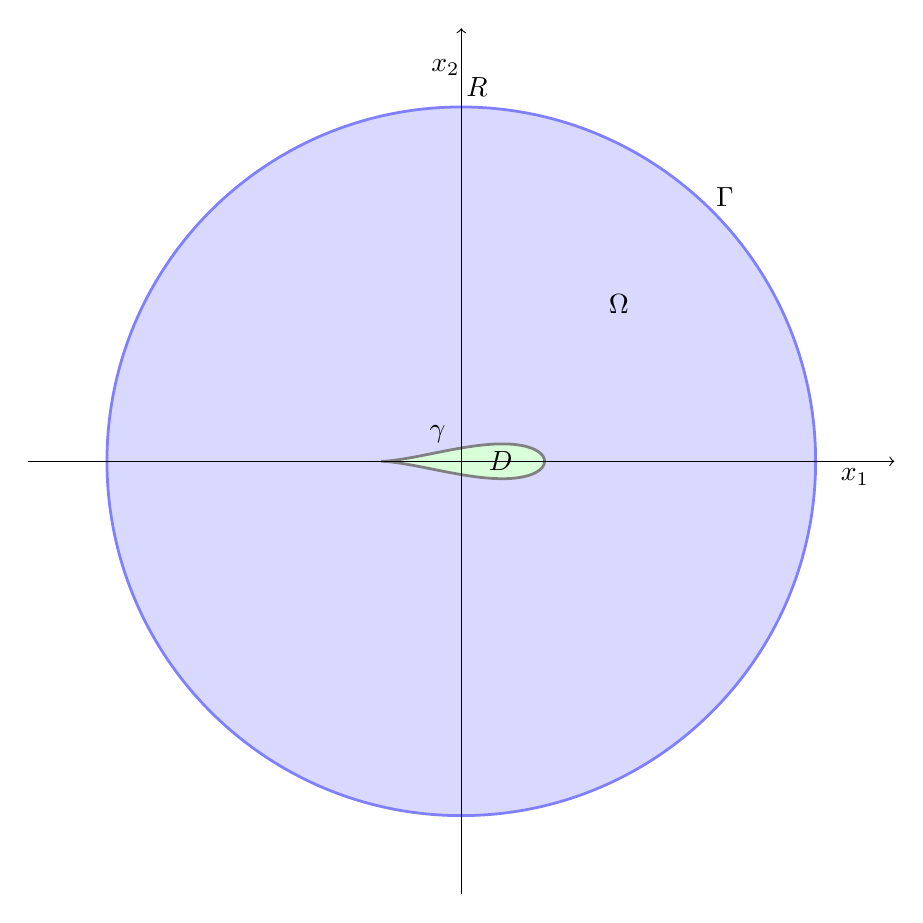
\begin{tikzpicture}[scale=1]

   \fill [blue!15] (0,0) circle (4.5);
   \draw [blue!50, line width=1pt] (0,0) circle (4.5);
% Параметры профиля Жуковского
\def\a{0.5} % Параметр, определяющий форму профиля
\def\c{0.1} % Смещение центра круга
\pgfmathsetmacro{\R}{\a + \c} % Радиус круга

% Построение профиля Жуковского
\fill[thick, green!15, smooth, variable=\t, domain=0:360, samples=200] 
    plot (%
        {\c + \R * cos(\t) + (\a^2) * (\c + \R * cos(\t)) / ((\c + \R * cos(\t))^2 + (\R * sin(\t))^2)},%
        {\R * sin(\t) - (\a^2) * (\R * sin(\t)) / ((\c + \R * cos(\t))^2 + (\R * sin(\t))^2)}%
    );
\draw[thick, black!50, line width=1pt, smooth, variable=\t, domain=0:360, samples=200] 
    plot (%
        {\c + \R * cos(\t) + (\a^2) * (\c + \R * cos(\t)) / ((\c + \R * cos(\t))^2 + (\R * sin(\t))^2)},%
        {\R * sin(\t) - (\a^2) * (\R * sin(\t)) / ((\c + \R * cos(\t))^2 + (\R * sin(\t))^2)}%
    );


   \draw[->] (-5.5,0) -- (5.5,0);
   \draw[->] (0,-5.5) -- (0,5.5);
   \draw(5,-0.2) node {$x_1$};   
   \draw(-0.2,5) node {$x_2$};  
   \draw(3.35,3.35) node {$\Gamma$};
   \draw(0.5,0.) node {$D$};  
   \draw(-0.3,0.35) node {$\gamma$};
   \draw(2,2) node {$\Omega$};
   \draw(0.2,4.75) node {$R$};

 \end{tikzpicture}
\end{figure}


\end{document}